% Practice Test 07 — Indiana Edition
% Questions: 30 (18 MC + 12 SA)
% Generated by scripts/generate_practice_tests.py

\begin{practiceQuestion}{1-3-q23}{sa}
\begin{questionText}
Two quantities are proportional with $k = 7$. If $y = 56$, what is $x$?
\end{questionText}
\correctAnswer{$x = 8$}
\explanation{$y = kx$ so $56 = 7x$, giving $x = 56 \div 7 = 8$.}
\end{practiceQuestion}

\begin{practiceQuestion}{1-5-q09}{mc}
\begin{questionText}
The point $(1, r)$ on a proportional graph represents:
\end{questionText}
\choiceA{The total amount}
\choiceB{The unit rate}
\choiceC{The number of units}
\choiceD{The $y$-intercept}
\correctAnswer{B}
\explanation{At $x = 1$, $y = k \times 1 = k$. So the $y$-value at $x = 1$ is the unit rate.}
\end{practiceQuestion}

\begin{practiceQuestion}{1-6-q29}{gsa}
\begin{questionText}
The double number line below relates inches on a blueprint to actual feet. A hallway measures $3.5$ inches on the blueprint. What is the actual length?

\begin{center}
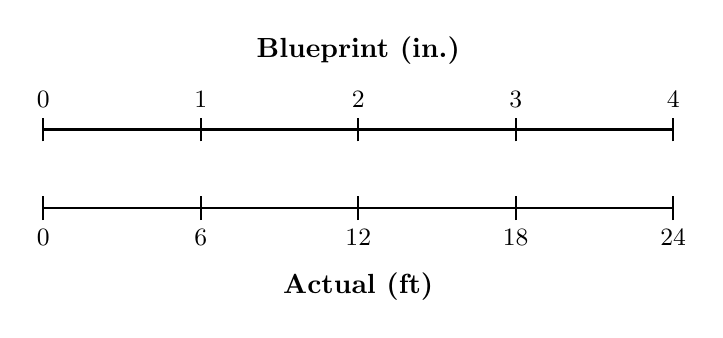
\begin{tikzpicture}[scale=1.0]
  % Top: blueprint inches
  \draw[thick] (0,1) -- (8,1);
  \foreach \x/\lab in {0/$0$, 2/$1$, 4/$2$, 6/$3$, 8/$4$} {
    \draw[thick] (\x,0.85) -- (\x,1.15);
    \node[above] at (\x,1.15) {\small \lab};
  }
  \node[above] at (4,1.7) {\textbf{Blueprint (in.)}};
  % Bottom: actual feet
  \draw[thick] (0,0) -- (8,0);
  \foreach \x/\lab in {0/$0$, 2/$6$, 4/$12$, 6/$18$, 8/$24$} {
    \draw[thick] (\x,-0.15) -- (\x,0.15);
    \node[below] at (\x,-0.15) {\small \lab};
  }
  \node[below] at (4,-0.7) {\textbf{Actual (ft)}};
\end{tikzpicture}
\end{center}
\end{questionText}
\correctAnswer{$21$ feet}
\explanation{Scale: $1$ inch $= 6$ feet. For $3.5$ inches: $6 \times 3.5 = 21$ feet.}
\end{practiceQuestion}

\begin{practiceQuestion}{2-2-q27}{gmc}
\begin{questionText}
The bar model below represents a whole amount. Use the model to find what percent the shaded part is of the whole.

\begin{center}
\begin{tikzpicture}[scale=0.65]
  % Whole bar divided into 8 equal parts, 3 shaded
  \foreach \i in {0,...,7} {
    \draw[thick] (\i*1,0) rectangle (\i*1+1,0.8);
  }
  \fill[funBlue!40] (0,0) rectangle (1,0.8);
  \fill[funBlue!40] (1,0) rectangle (2,0.8);
  \fill[funBlue!40] (2,0) rectangle (3,0.8);
  \foreach \i in {0,...,7} {
    \draw[thick] (\i*1,0) rectangle (\i*1+1,0.8);
  }
  \draw[thick,<->] (0,-0.4) -- (3,-0.4) node[midway,below,font=\small] {$45$};
  \draw[thick,<->] (0,-1.1) -- (8,-1.1) node[midway,below,font=\small] {Whole $= {?}$};
  \node[above,font=\small] at (1.5,0.8) {Shaded};
\end{tikzpicture}
\end{center}

If each section has the same value and there are $8$ equal sections total, what percent is shaded?
\end{questionText}
\choiceA{$25\%$}
\choiceB{$33\%$}
\choiceC{$37.5\%$}
\choiceD{$45\%$}
\correctAnswer{C}
\explanation{$3$ out of $8$ sections are shaded. $\frac{3}{8} = \frac{p}{100}$ → $p = 37.5\%$.}
\end{practiceQuestion}

\begin{practiceQuestion}{2-5-q19}{sa}
\begin{questionText}
A dinner bill is $\$64$. You leave an $18\%$ tip. How much is the tip?
\end{questionText}
\correctAnswer{$\$11.52$}
\explanation{$64 \times 0.18 = \$11.52$.}
\end{practiceQuestion}

\begin{practiceQuestion}{2-7-q21}{sa}
\begin{questionText}
A baker expected to make $80$ cookies from a recipe but made $72$. What is the percent error (rounded to the nearest tenth)?
\end{questionText}
\correctAnswer{$\approx 11.1\%$}
\explanation{$\frac{|80 - 72|}{72} \times 100 = \frac{8}{72} \times 100 \approx 11.1\%$.}
\end{practiceQuestion}

\begin{practiceQuestion}{3-1-q12}{mc}
\begin{questionText}
The temperature at noon was $5°$C. By midnight it was $-5°$C. What is the relationship between these temperatures?
\end{questionText}
\choiceA{They are equal}
\choiceB{They are opposites}
\choiceC{Midnight was warmer}
\choiceD{Their absolute values are different}
\correctAnswer{B}
\explanation{$5$ and $-5$ are the same distance from $0$ but on opposite sides of the number line. They are opposites.}
\end{practiceQuestion}

\begin{practiceQuestion}{3-2-q04}{mc}
\begin{questionText}
What is $9 + (-14)$?
\end{questionText}
\choiceA{$23$}
\choiceB{$-23$}
\choiceC{$-5$}
\choiceD{$5$}
\correctAnswer{C}
\explanation{Different signs: $14 - 9 = 5$. The larger absolute value ($14$) is negative, so the answer is $-5$.}
\end{practiceQuestion}

\begin{practiceQuestion}{4-2-q16}{mc}
\begin{questionText}
Which expression is equivalent to $-x + 8 + 4x - 5$?
\end{questionText}
\choiceA{$3x + 3$}
\choiceB{$5x + 3$}
\choiceC{$-3x + 3$}
\choiceD{$3x + 13$}
\correctAnswer{A}
\explanation{Combine variable terms: $-x + 4x = 3x$. Combine constants: $8 - 5 = 3$. Result: $3x + 3$.}
\end{practiceQuestion}

\begin{practiceQuestion}{4-3-q08}{mc}
\begin{questionText}
Expand and simplify $2(x + 3) + 5$.
\end{questionText}
\choiceA{$2x + 8$}
\choiceB{$2x + 11$}
\choiceC{$2x + 10$}
\choiceD{$7x + 3$}
\correctAnswer{B}
\explanation{Expand: $2x + 6$. Add $5$: $2x + 6 + 5 = 2x + 11$.}
\end{practiceQuestion}

\begin{practiceQuestion}{5-4-q13}{mc}
\begin{questionText}
A shirt is on sale for $\dfrac{2}{3}$ of its original price. After using a $\$5$ coupon, you pay $\$15$. What equation finds the original price $p$?
\end{questionText}
\choiceA{$\dfrac{2}{3}p + 5 = 15$}
\choiceB{$p - \dfrac{2}{3} - 5 = 15$}
\choiceC{$\dfrac{2}{3}p - 5 = 15$}
\choiceD{$\dfrac{2}{3}(p - 5) = 15$}
\correctAnswer{C}
\explanation{Sale price is $\frac{2}{3}p$. After the $\$5$ coupon: $\frac{2}{3}p - 5 = 15$.}
\end{practiceQuestion}

\begin{practiceQuestion}{5-5-q17}{mc}
\begin{questionText}
Which inequality means ``no more than $25$''?
\end{questionText}
\choiceA{$x > 25$}
\choiceB{$x \geq 25$}
\choiceC{$x < 25$}
\choiceD{$x \leq 25$}
\correctAnswer{D}
\explanation{``No more than $25$'' means $25$ or fewer: $x \leq 25$.}
\end{practiceQuestion}

\begin{practiceQuestion}{5-6-q20}{sa}
\begin{questionText}
Solve $-5x + 15 \geq 30$. Describe the graph.
\end{questionText}
\correctAnswer{$x \leq -3$; closed circle at $-3$, shade left}
\explanation{Subtract $15$: $-5x \geq 15$. Divide by $-5$ and flip: $x \leq -3$. Closed circle at $-3$, shade left.}
\end{practiceQuestion}

\begin{practiceQuestion}{6-1-q26}{gmc}
\begin{questionText}
A blueprint of a house is shown below. The scale is $1$ cm $= 5$ m. What is the actual length of the living room?

\begin{center}
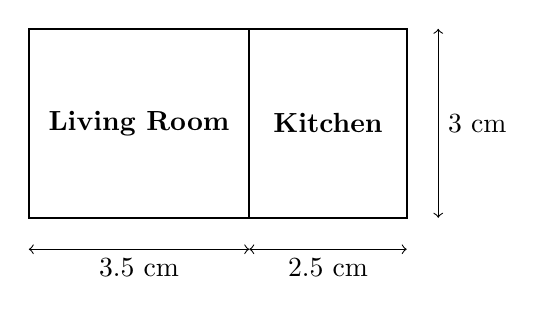
\begin{tikzpicture}[scale=0.8]
  \draw[thick] (0,0) rectangle (6,3);
  \draw[thick] (3.5,0) -- (3.5,3);
  \node at (1.75,1.5) {\textbf{Living Room}};
  \node at (4.75,1.5) {\textbf{Kitchen}};
  \draw[<->] (0,-0.5) -- (3.5,-0.5);
  \node[below] at (1.75,-0.5) {$3.5$ cm};
  \draw[<->] (3.5,-0.5) -- (6,-0.5);
  \node[below] at (4.75,-0.5) {$2.5$ cm};
  \draw[<->] (6.5,0) -- (6.5,3);
  \node[right] at (6.5,1.5) {$3$ cm};
\end{tikzpicture}
\end{center}
\end{questionText}
\choiceA{$3.5$ m}
\choiceB{$12.5$ m}
\choiceC{$15$ m}
\choiceD{$17.5$ m}
\correctAnswer{D}
\explanation{The living room is $3.5$ cm on the drawing. Actual length: $3.5 \times 5 = 17.5$ m.}
\end{practiceQuestion}

\begin{practiceQuestion}{6-3-q29}{gsa}
\begin{questionText}
Look at the triangle below. Two angles are given. Can this triangle exist? If so, what is the third angle?

\begin{center}
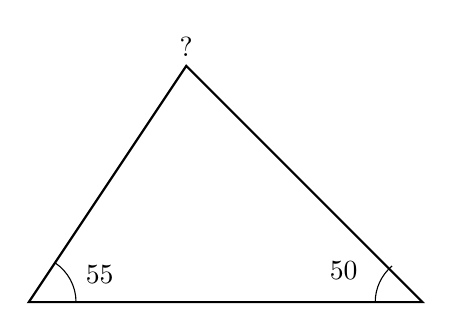
\begin{tikzpicture}[scale=1]
  \draw[thick] (0,0) -- (5,0) -- (2,3) -- cycle;
  \draw (0.6,0) arc[start angle=0,end angle=56,radius=0.6];
  \node at (0.9,0.35) {$55°$};
  \draw (4.4,0) arc[start angle=180,end angle=130,radius=0.6];
  \node at (4,0.4) {$50°$};
  \node[above] at (2,3) {$?$};
\end{tikzpicture}
\end{center}
\end{questionText}
\correctAnswer{Yes; the third angle is $75°$}
\explanation{$180° - 55° - 50° = 75°$. The angles sum to $180°$, so the triangle can exist. The third angle is $75°$.}
\end{practiceQuestion}

\begin{practiceQuestion}{6-4-q30}{gsa}
\begin{questionText}
The diagram shows a triangle with the three side lengths labeled. Does it satisfy the triangle inequality? If so, is it unique?

\begin{center}
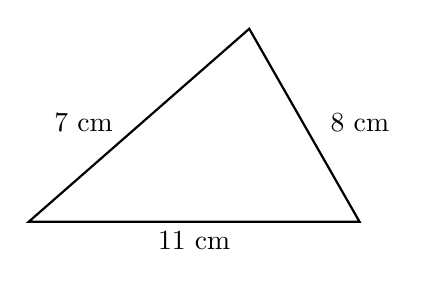
\begin{tikzpicture}[scale=0.7]
  \draw[thick] (0,0) -- (6,0) -- (4,3.5) -- cycle;
  \node[below] at (3,0) {$11$ cm};
  \node[left] at (1.7,1.8) {$7$ cm};
  \node[right] at (5.3,1.8) {$8$ cm};
\end{tikzpicture}
\end{center}
\end{questionText}
\correctAnswer{Yes, it satisfies the inequality and is unique}
\explanation{$7 + 8 = 15 > 11$ \checkmark, $7 + 11 = 18 > 8$ \checkmark, $8 + 11 = 19 > 7$ \checkmark. SSS with valid lengths produces exactly one unique triangle.}
\end{practiceQuestion}

\begin{practiceQuestion}{6-5-q24}{sa}
\begin{questionText}
Is it possible to get a circular cross-section from a rectangular prism? Explain.
\end{questionText}
\correctAnswer{No}
\explanation{A rectangular prism has only flat faces and straight edges. All cross-sections are polygons (triangles, rectangles, pentagons, hexagons). A circular cross-section requires a curved surface.}
\end{practiceQuestion}

\begin{practiceQuestion}{6-6-q19}{sa}
\begin{questionText}
Find the complement of $67°$.
\end{questionText}
\correctAnswer{$23°$}
\explanation{$90° - 67° = 23°$.}
\end{practiceQuestion}

\begin{practiceQuestion}{6-7-q13}{mc}
\begin{questionText}
After reflecting point $K$ over the $x$-axis, the image is $K'(4, -3)$. What were the original coordinates of $K$?
\end{questionText}
\choiceA{$(4, 3)$}
\choiceB{$(-4, -3)$}
\choiceC{$(-4, 3)$}
\choiceD{$(4, -3)$}
\correctAnswer{A}
\explanation{Reflection over the $x$-axis negates $y$. To reverse: $K'(4, -3) \to K(4, 3)$.}
\end{practiceQuestion}

\begin{practiceQuestion}{7-3-q16}{mc}
\begin{questionText}
A student says the area of a circle with radius $6$ cm is $37.68$ cm$^2$. What mistake did the student most likely make?
\end{questionText}
\choiceA{Used diameter instead of radius}
\choiceB{Calculated circumference instead of area}
\choiceC{Forgot to square the radius}
\choiceD{Divided by $2$ instead of squaring}
\correctAnswer{B}
\explanation{$C = 2\pi r = 2 \times 3.14 \times 6 = 37.68$. The student found circumference, not area. The area is $3.14 \times 36 = 113.04$ cm$^2$.}
\end{practiceQuestion}

\begin{practiceQuestion}{7-4-q09}{mc}
\begin{questionText}
A banner is shaped like a rectangle $18$ in by $6$ in with a triangle cut from one end. The triangle has a base of $6$ in and a height of $4$ in. What is the area of the banner?
\end{questionText}
\choiceA{$84$ in$^2$}
\choiceB{$96$ in$^2$}
\choiceC{$108$ in$^2$}
\choiceD{$120$ in$^2$}
\correctAnswer{B}
\explanation{Rectangle: $18 \times 6 = 108$ in$^2$. Triangle: $\frac{1}{2} \times 6 \times 4 = 12$ in$^2$. Banner: $108 - 12 = 96$ in$^2$.}
\end{practiceQuestion}

\begin{practiceQuestion}{7-5-q12}{mc}
\begin{questionText}
A storage box is in the shape of a cube with side $12$ inches. What is its surface area?
\end{questionText}
\choiceA{$144$ in$^2$}
\choiceB{$432$ in$^2$}
\choiceC{$864$ in$^2$}
\choiceD{$1728$ in$^2$}
\correctAnswer{C}
\explanation{$SA = 6s^2 = 6 \times 144 = 864$ in$^2$.}
\end{practiceQuestion}

\begin{practiceQuestion}{7-6-q08}{mc}
\begin{questionText}
A storage container is $2$ ft long, $1.5$ ft wide, and $3$ ft tall. How many cubic feet can it hold?
\end{questionText}
\choiceA{$6$ ft$^3$}
\choiceB{$6.5$ ft$^3$}
\choiceC{$9$ ft$^3$}
\choiceD{$10$ ft$^3$}
\correctAnswer{C}
\explanation{$V = 2 \times 1.5 \times 3 = 9$ ft$^3$.}
\end{practiceQuestion}

\begin{practiceQuestion}{8-1-q26}{gmc}
\begin{questionText}
A student surveyed $50$ classmates about their favorite fruit. The results are shown in the bar graph below.

\begin{center}
\begin{tikzpicture}[scale=0.7]
  \draw[thick,->] (0,0) -- (0,6.5) node[above]{\small Number of Students};
  \draw[thick,->] (0,0) -- (8.5,0);
  % bars
  \fill[funBlue!70] (0.5,0) rectangle (1.5,4);
  \fill[funGreen!70] (2.5,0) rectangle (3.5,3);
  \fill[funOrange!70] (4.5,0) rectangle (5.5,2);
  \fill[funRed!70] (6.5,0) rectangle (7.5,1);
  % labels
  \node[below] at (1,0) {\small Apple};
  \node[below] at (3,0) {\small Banana};
  \node[below] at (5,0) {\small Orange};
  \node[below] at (7,0) {\small Grape};
  % y-axis ticks
  \foreach \y in {1,2,3,4,5,6} {
    \draw (-0.1,\y) -- (0.1,\y);
    \node[left] at (0,\y) {\small $\y\times5$};
  }
  % values on bars
  \node[above] at (1,4) {\small $20$};
  \node[above] at (3,3) {\small $15$};
  \node[above] at (5,2) {\small $10$};
  \node[above] at (7,1) {\small $5$};
\end{tikzpicture}
\end{center}

If there are $500$ students in the school, predict how many prefer apples.
\end{questionText}
\choiceA{$20$}
\choiceB{$100$}
\choiceC{$200$}
\choiceD{$250$}
\correctAnswer{C}
\explanation{$\frac{20}{50} = 40\%$ prefer apples. $40\%$ of $500 = 200$.}
\end{practiceQuestion}

\begin{practiceQuestion}{8-3-q13}{mc}
\begin{questionText}
The difference between the means of two groups is $10$. The MAD for each group is $2$. How many MADs apart are the means?
\end{questionText}
\choiceA{$2$}
\choiceB{$5$}
\choiceC{$10$}
\choiceD{$20$}
\correctAnswer{B}
\explanation{$\frac{10}{2} = 5$ MADs apart.}
\end{practiceQuestion}

\begin{practiceQuestion}{8-4-q15}{mc}
\begin{questionText}
Why is it important to use multiple measures (mean, median, range, IQR, MAD) when comparing two groups?
\end{questionText}
\choiceA{One measure tells the complete story}
\choiceB{Using more measures wastes time}
\choiceC{Different measures reveal different aspects of the data}
\choiceD{All measures always give the same conclusion}
\correctAnswer{C}
\explanation{Mean and median show center; range, IQR, and MAD show spread. Together they give a complete picture.}
\end{practiceQuestion}

\begin{practiceQuestion}{8-7-q19}{sa}
\begin{questionText}
A frequency table shows: Soccer $15$, Basketball $20$, Tennis $10$, Swimming $5$. What is the total and what percent play basketball?
\end{questionText}
\correctAnswer{Total $= 50$; Basketball $= 40\%$}
\explanation{$15+20+10+5 = 50$. Basketball: $\frac{20}{50} = 40\%$.}
\end{practiceQuestion}

\begin{practiceQuestion}{9-4-q30}{gsa}
\begin{questionText}
The table below shows a probability model for a game spinner. One probability is missing. Find the missing probability for outcome D.

\begin{center}
\begin{tabular}{|c|c|}
\hline
\textbf{Outcome} & \textbf{Probability} \\
\hline
A & $0.30$ \\
\hline
B & $0.25$ \\
\hline
C & $0.15$ \\
\hline
D & ? \\
\hline
\end{tabular}
\end{center}
\end{questionText}
\correctAnswer{$0.30$}
\explanation{$P(D) = 1 - (0.30 + 0.25 + 0.15) = 1 - 0.70 = 0.30$.}
\end{practiceQuestion}

\begin{practiceQuestion}{9-6-q06}{mc}
\begin{questionText}
Two dice are rolled. What is the probability that both dice show the same number (doubles)?
\end{questionText}
\choiceA{$\frac{1}{36}$}
\choiceB{$\frac{1}{12}$}
\choiceC{$\frac{1}{6}$}
\choiceD{$\frac{1}{3}$}
\correctAnswer{C}
\explanation{Doubles: $(1,1), (2,2), (3,3), (4,4), (5,5), (6,6)$ — that is $6$ out of $36$. $P = \frac{6}{36} = \frac{1}{6}$.}
\end{practiceQuestion}

\begin{practiceQuestion}{9-7-q25}{sa}
\begin{questionText}
A student runs $200$ simulation trials for an event with theoretical probability $\frac{1}{4}$. They observe the event $54$ times. What is the experimental probability? Is it close to the theoretical value?
\end{questionText}
\correctAnswer{$0.27$; yes, it is close to $0.25$}
\explanation{$P = \frac{54}{200} = 0.27$. Theoretical $= 0.25$. The difference of $0.02$ is small, especially with $200$ trials.}
\end{practiceQuestion}
